\documentclass[12pt]{article}
%\usepackage{graphicx}
\usepackage[pdftex]{graphicx}
\usepackage{fancyhdr}
\usepackage[latin1]{inputenc}
\usepackage{moreverb}
\usepackage{amssymb}
\usepackage{caption}
\usepackage{hyperref}
\usepackage{subcaption}
\usepackage{longtable}
\usepackage{draftwatermark}
%\usepackage[sectionbib]{natbib}
\usepackage[english]{babel}
\pagestyle{fancy}
\begin{document}
\fancyhead[LE,LO]{
\includegraphics[height=13pt]{molflow.png}}
\fancyhead[CE,CO]{}
\fancyhead[RE,RO]{}
\fancyfoot[LO,LE]{}
\fancyfoot[RO,RE]{}
\fancyfoot[CO,CE]{\thepage}
\renewcommand{\footrulewidth}{0.4pt}
\renewcommand{\headrulewidth}{0.4pt}


\begin{titlepage}
	    
\includegraphics[width=0.3\textwidth]{molflow.png}
  \begin{flushright}
    \noindent\rule{\textwidth}{2pt}
    \vspace{1cm}
    \begin{large}
	   Calibration of Odin-SMR measurements:\\
           -an overview of the calibration- database and
            routine, and the processing system\\
    \end{large}
      \vspace{1cm}
    \today\\
    \noindent\rule{\textwidth}{2pt}
    \vspace{1cm}\\
    \begin{minipage}[t]{0.3\textwidth}
    \end{minipage}%
    \begin{minipage}[t]{0.30\textwidth}
	Joakim M\"{o}ller\\
        Bengt Rydberg
    \end{minipage}%
    \begin{minipage}[t]{0.4\textwidth}
      \begin{flushright}
        bengt.rydberg@molflow.com
        joakim.moller@molflow.com
      \end{flushright}
\end{minipage}
  \vspace{8cm}
\end{flushright}
\end{titlepage}

%\thispagestyle{empty}
%\newpage
\tableofcontents
\thispagestyle{empty}
\newpage
\setcounter{page}{1}
\section{Overview}
A processing system for the calibration of data 
(from level0-files to calibrated level1b-data;
geolocated, frequency, and intensity calibrated data)
from the auto-correlators of Odin-SMR has been developed.

This document describes the processing system,
the main programs of the processing system,
the calibration routine applied,  
the installation and configuration procedure.
A key component of the processing system is a database 
called \(odin\), which contains all relevant data
and is also used for keeping track of the processing of data.
The \(odin\) database is described, and useful examples
how to export data from the various tables of \(odin\) are given.


\clearpage
\newpage


\section{The Odin database}
\subsection{Overview}
Various types of data 
(e.g. auto-correlator-, attitude-, housekeeping-data) is used for the 
calibration of Odin-SMR measurements.
A database, with tables of data from the various sources at different levels
(level0 to level1b), 
called \(odin\) has been developed, to keep track of all
data and for the processing of data.
\(odin\) is a PostgreSQL database, see e.g. \url{http://www.postgresql.org/docs/} for online PostgreSQL documentation.
How to start a PostgreSQL interactive terminal is described in 
Sect.~\ref{sec:usermanual}, and how to 
acces the \(odin\) database using Matlab
and Python is described in Sect.~\ref{sec:matlab} and~\ref{sec:python},
respectively. 
Section~\ref{sec:officialexport} describes the export of the
official level1b-product.

\subsection{Database tables}
The database \(odin\) consists of 17 tables (see Table~\ref{table:odin_tables} ) .\\ 
-Five tables are used for the processing of data (see Table~\ref{table:processing} ).\\
-Four tables contains basic level0-data (see Table~\ref{table:level0} ).\\
-Three tables contains processed level0-data (see Table~\ref{table:level1} ).\\ 
-Two tables contains processed level1-data (see Table~\ref{table:level1b} ).\\ 
-Two tables contains processed level1b-data (see Table~\ref{table:level1c} ).\\ 
The various tables are described in the following sections.


\begin{table}[!htb]
\captionsetup{font=scriptsize}
\begin{scriptsize}
   \centering
    \caption{Tables of tables of the odin database}
    \label{table:odin_tables}
    \begin{subtable}{.9\linewidth}
    \captionsetup{font=scriptsize}
     \caption{Tables used for the processing of data}
     \label{table:processing}
      \centering
        \begin{tabular}{ll}
          \hline\hline
Table-name & Description\\ [0.5ex]
\hline
level0\underline{ }files  & -\\
level0\underline{ }files\underline{ }in\underline{ }process  &  -\\
level0\underline{ }files\underline{ }imported  &  -\\
processed  &  -\\
in\underline{ }process  &  -\\[1ex]
\hline
 
        \end{tabular}
    \end{subtable}%
    \newline
    \newline

    \begin{subtable}{.9\linewidth}
     \captionsetup{font=scriptsize}
       \caption{Tables containing level0-data}
     \label{table:level0}
      \centering
        \begin{tabular}{ll}
          \hline\hline
Table-name & Description\\ [0.5ex]
\hline
ac\underline{ }level0  & -\\
attitude\underline{ }level0 &  -\\
shk\underline{ }level0  &  -\\
fba\underline{ }level0  &  -\\[1ex]
\hline
  
        \end{tabular}
    \end{subtable}
   \newline
   \newline

   \begin{subtable}{.9\linewidth}
     \captionsetup{font=scriptsize}
       \caption{Tables containing processed level0-data}
     \label{table:level1}
      \centering     
        \begin{tabular}{ll}
      \hline\hline
Table-name & Description\\ [0.5ex]
\hline
ac\underline{ }level1a  & -\\
attitude\underline{ }level1 &  -\\
shk\underline{ }level1  &  -\\
\hline
      
        \end{tabular}
    \end{subtable}
   \newline
   \newline

 \begin{subtable}{.9\linewidth}
     \captionsetup{font=scriptsize}
       \caption{Tables containing processed level1-data}
     \label{table:level1b}
      \centering     
        \begin{tabular}{ll}
           \hline\hline
Table-name & Description\\ [0.5ex]
\hline
ac\underline{ }level1b  &  -\\
ac\underline{ }cal\underline{ }level1b  &  -\\
\hline
 
        \end{tabular}
    \end{subtable}
   \newline
\newline

 \begin{subtable}{.9\linewidth}
     \captionsetup{font=scriptsize}
      \caption{Tables containing processed level1b-data}
     \label{table:level1c}
      \centering     
        \begin{tabular}{ll}
          \hline\hline
Table-name & Description\\ [0.5ex]
\hline
ac\underline{ }level1b\underline{ }average  &  -\\
ac\underline{ }cal\underline{ }level1c  &  -\\[1ex]
\hline
  
        \end{tabular}
    \end{subtable}
 
   

 
\end{scriptsize}
\end{table}


\clearpage
\newpage

\subsubsection{Tables used for processing of data}
\label{sec:processingtables}
Five tables are used for the processing of data (see Table~\ref{table:processfile} ).
The most basic table is level0\underline{ }files, which contains
rows of filenames of all relevant odin level0-files,
and the measurement date of the first row of data of each file.
The type of files contained in level0\underline{ }files are
ac1-files, ac2-files, attitude-files, shk-files, and fba-files.

The rows in tables level0\underline{ }files\underline{ }imported and  
level0\underline{ }files\underline{ }in\underline{ }process,
contains information on from which level0-files data have,
or are scheduled to be, imported into the level0-data tables.
That is, if a given filename exists in the table 
level0\underline{ }files\underline{ }imported, data from
this file has been imported into a database table, and 
the column created tells when this was done. 
 
The rows in tables processed and in\underline{ }process 
describes which ac-files that have been calibrated
or are scheduled to be calibrated.
The calibration routine is scan-based, but the processing-system
is ``file-based'' in the following meaning. 
The processing system can identify that data
from a number of ac-files not yet have been calibrated,
by querying these tables, and then decide
to calibrate all scans that starts within a given file,
according to the calibration routine described in Sect.~\ref{sec:calibration}.

\begin{table}[!htb]
 \begin{scriptsize}
  \centering
    \captionsetup{font=scriptsize}
    \caption{Tables used for the processing}
    \label{table:processfile}
    \begin{subtable}{.9\linewidth}
     \captionsetup{font=scriptsize}
      \centering
      \caption{level0\underline{ }files}
      \label{table:level0f}
        \begin{tabular}{l l l}
         \hline\hline
Column & Type & Description \\ [0.5ex]
\hline
file (key)                     & character varying                   & -\\
measurement\underline{ }date   & date                        & -\\
created                        & timestamp                   & -\\[1ex]
\hline   
        \end{tabular}
    \end{subtable}%
    \newline
    \newline

    \begin{subtable}{.9\linewidth}
     \captionsetup{font=scriptsize}
      \centering
      \caption{level0\underline{ }files\underline{ }in\underline{ }process}
      \label{table:level0fip}
        \begin{tabular}{l l l}
\hline\hline
Column & Type & Description \\ [0.5ex]
\hline
file (key)                     & character varying                  & -\\
created                        & timestamp                   & -\\[1ex]
\hline            
        \end{tabular}
    \end{subtable}%
    \newline
    \newline

    \begin{subtable}{.9\linewidth}
     \captionsetup{font=scriptsize}
      \centering
         \caption{level0\underline{ }files\underline{ }processed}
      \label{table:level0fp}
        \begin{tabular}{l l l}
\hline\hline
Column & Type & Description \\ [0.5ex]
\hline
file (key)                     & character varying                  & -\\
created                        & timestamp                   & -\\[1ex]
\hline
            
        \end{tabular}
    \end{subtable}%
    \newline
    \newline

    \begin{subtable}{.9\linewidth}
     \captionsetup{font=scriptsize}
      \centering
       \caption{in\underline{ }process}
      \label{table:in_process}
        \begin{tabular}{l l l}
 \hline\hline
Column & Type & Description \\ [0.5ex]
\hline
file (key)                     & character varying                  & -\\
version                        & integer                     & -\\
created                        & timestamp                   & -\\[1ex]
\hline
           
        \end{tabular}
    \end{subtable}%
    \newline
    \newline

    \begin{subtable}{.9\linewidth}
     \captionsetup{font=scriptsize}
      \centering
        \caption{processed}
      \label{table:processed}
        \begin{tabular}{l l l}
          \hline\hline
Column & Type & Description \\ [0.5ex]
\hline
file (key)                     & character varying                  & -\\
total\underline{ }scans        & integer                     & -\\
info                           & character varying                   & -\\
version                        & integer                     & -\\
created                        & timestamp                   & -\\[1ex]
\hline
            
        \end{tabular}
    \end{subtable}%
    \newline
    \newline
\end{scriptsize}    
\end{table}



\clearpage
\newpage


\subsubsection{Tables containing level0-data}
Four tables (see Table~\ref{table:level0data} ) contains basic ''unprocessed''  
level0-data, and these are: 
ac\underline{ }level0, shk\underline{ }level0, attitude\underline{ }level0,
and fba\underline{ }level0.
A common key column in these tables is satellite time word (stw),
although the data in the various tables have different time resolution.
There is in general no match in stw across these tables, except
for the ac\underline{ }level0 and fba\underline{ }level0 tables
(see  further in Sect.~\ref{sec:scanid}).


\begin{table}
 \begin{tiny}    
   \captionsetup{font=scriptsize}
    \caption{Tables containing level0-data}
     \label{table:level0data}
    \begin{subtable}{.9\linewidth}
      \captionsetup{font=scriptsize}
      \centering
       \label{table:ac0}
\caption{ac\underline{ }level0}
      \begin{tabular}{l l l}
\hline
\hline
Column & Type & Description \\ [0.5ex]
\hline
stw (key)            & bigint                                &  - \\
backend (key)        & ('AC1','AC2')                         & -\\
frontend             & ('549','495','572','555','SPL','119') & -\\
sig\underline{ }type & ('REF','SIG')                         & -\\
ssb\underline{ }att  & integer[]                             & -\\
ssb\underline{ }fq   & integer[]                             & the four lo freq. of the ssb modules\\
prescaler            & integer                               & -\\
inttime              & real                                  & -\\
mode                 & integer                               & correlator configuration\\
acd\underline{ }mon  & bytea, shape=(8,2),dtype='float64'    & monitor data\\
cc                   & bytea, shape=(8,96),dtype='float64'   & correlation coefficients\\
file                     & character varying                  & -\\
created                        & timestamp                   & -\\[1ex]
\hline
\end{tabular}

    \end{subtable}%
\newline
\newline

    \begin{subtable}{.9\linewidth}
      \centering
       \captionsetup{font=scriptsize}
        \label{table:fba0}
\caption{fba\underline{ }level0}
\begin{tabular}{l l l}
\hline
\hline
Column & Type & Description \\ [0.5ex]
\hline
stw (key) & bigint & - \\
mech\underline{ }type & ('SK1','SK2','CAL') & -\\
file                      & character varying                  & -\\
created                        & timestamp                   & -\\[1ex]
\hline
\end{tabular}
    \end{subtable} 
 \newline
\newline

\begin{subtable}{.9\linewidth}
      \centering
       \captionsetup{font=scriptsize}
       \label{table:att0}
\caption{attitude\underline{ }level0}
\begin{tabular}{l l l}
\hline
\hline
Column & Type & Description \\ [0.5ex]
\hline
stw (key) & bigint             & - \\
soda (key) & integer             & - \\
year     & integer            & -\\
mon     & integer            & -\\
day     & integer            & -\\
hour    & integer            & -\\
min     & integer            & -\\
secs    & double precision   & -\\
orbit   & double precision   & -\\ 
qt      & double precision[] & qtarget (4-vector)\\
qa      & double precision[] & qachieved (4-vector)\\
qe      & double precision[] & qerror (3-vector)\\
gps     & double precision[] & gps position and velocity (6-vector)\\
acs     & double precision   & -\\
file                      & character varying                   & -\\
created                        & timestamp                   & -\\[1ex]
\hline
\end{tabular}
    \end{subtable}
\newline
\newline

\begin{subtable}{.9\linewidth}
      \centering
       \captionsetup{font=scriptsize}
       \label{table:shk0}
\caption{shk\underline{ }level0}
\begin{tabular}{l l l}
\hline
\hline
Column & Type & Description \\ [0.5ex]
\hline
stw (key) & bigint & - \\
shk\underline{ }type (key) & ('LO495','LO549','LO555','LO572',  & lo freq.\\
 & 'SSB495','SSB549','SSB555','SSB572', & ssb tunings\\
 & 'mixC495','mixC549','mixC555','mixC572', & mixer current\\
 & 'imageloadA','imageloadB','hotloadA','hotloadB' & temperatures\\  
 & 'mixerA','mixerB','lnaA','lnaB' &  temperatures\\ 
 & '119mixerA','119mixerB','warmifA','warmifB') & temperatures  \\
shk\underline{ }value & real & -\\
file                      & character varying                   & -\\
created                        & timestamp                   & -\\[1ex]
\hline
\end{tabular}
    \end{subtable} 
 \end{tiny}    
\end{table}

\clearpage
\newpage


\subsubsection{Tables containing processed level0-data}
Three tables (see Table~\ref{table:level1data} ) contains processed 
level0-data,
and these are: attitude\underline{ }level1, shk\underline{ }level1, 
and ac\underline{ }level1a.
Data from the attitude\underline{ }level1 and shk\underline{ }level1 
tables have been
processed to match the stw (and frontend for shk\underline{ }level1) 
of the rows in the  table ac\underline{ }level0.
For the split modes (frontend='SPL' in the ac\underline{ }level0 table)
the backend receives input from two frontends (AC1 will hold 495 data 
in its lower half and 549 in its upper half, AC2 will hold 572 data in its
lower half and 555 in its upper half). That means for example, 
that for a split mode measurement using AC1, the table 
shk\underline{ }level1 will contain one row of 495 and one row of
549 data for a given stw and backend='AC1'.
The rows of the ac\underline{ }level1a table contain 
uncalibrated spectra in the frequency domain, which means that
a FFT-operation has been applied to the correlation coefficients found 
in the ac\underline{ }level0 table. 

\begin{table}
  \begin{tiny}
     \captionsetup{font=scriptsize}
    \caption{Tables containing processed level0-data}
    \label{table:level1data}
    \begin{subtable}{.9\linewidth}
      \captionsetup{font=scriptsize}
      \centering
      \label{table:ac1a}
\caption{ac\underline{ }level1a}

        \begin{tabular}{l l l}
\hline\hline
Column & Type & Description \\ [0.5ex]
\hline
stw (key)    & bigint         & - \\
backend (key) & ('AC1','AC2')  & -\\
spectra & bytea, shape=(112*8,),dtype='float64' & spectrum in the \\
& & frequency domain\\[1ex]
\hline
\end{tabular}

       
    \end{subtable}%
   \newline
   \newline

\begin{subtable}{.9\linewidth}
      \captionsetup{font=scriptsize}
      \centering
      \label{table:att1}
\caption{attitude\underline{ }level1}

       \begin{tabular}{l l l}
\hline\hline
Column & Type & Description \\ [0.5ex]
\hline
 stw (key)  & bigint             & - \\
 backend (key) & ('AC1','AC2')   & - \\
 soda (key) & integer            & - \\
 mjd        & double precision   & - \\  
 lst        & real               & - \\   
 orbit      & double precision   & - \\   
 latitude   & real               & - \\    
 longitude  & real               & - \\    
 altitude   & real               & - \\    
 skybeamhit & integer            & - \\    
 ra2000     & real               & - \\    
 dec2000    & real               & - \\    
 vsource    & real               & - \\    
 qtarget    & double precision[] & - \\ 
 qachieved  & double precision[] & - \\ 
 qerror     & double precision[] & - \\ 
 gpspos     & double precision[] & - \\    
 gpsvel     & double precision[] & - \\  
 sunpos     & double precision[] & - \\  
 moonpos    & double precision[] & - \\  
 sunzd      & real               & - \\  
 vgeo       & real               & - \\ 
 vlsr       & real               & - \\ 
 alevel     & integer            & -\\[1ex]
\hline
\end{tabular}
 
       
    \end{subtable}%
   \newline
   \newline

   \begin{subtable}{.9\linewidth}
      \captionsetup{font=scriptsize}
      \centering
      \label{table:shk1}
\caption{shk\underline{ }level1}

        \begin{tabular}{l l l}
\hline\hline
Column & Type & Description \\ [0.5ex]
\hline
 stw (key)       & bigint           & - \\
 backend (key)   & ('AC1','AC2')    & -\\ 
 frontendsplit (key) & ('549','495','572','555','119') & -\\
 lo         & real             & -\\ 
 ssb        & real             & -\\ 
 mixc       & real             & -\\  
 imageloada & real             & -\\
 imageloadb & real             & -\\
 hotloada   & real             & -\\ 
 hotloadb   & real             & -\\
 mixera     & real             & -\\
 mixerb     & real             & -\\
 lnaa       & real             & -\\
 lnab       & real             & -\\
 mixer119a  & real             & -\\
 mixer119b  & real             & -\\
 warmifa    & real             & -\\
 warmifb    & real             & -\\[1ex]
\hline
\end{tabular}

       
    \end{subtable}%
 

 \end{tiny}
\end{table}




\clearpage
\newpage

\subsubsection{Tables containing processed level1-data}
The tables ac\underline{ }level1b (Table~\ref{table:ac1b1})
 and ac\underline{ }cal\underline{ }level1b (Table~\ref{table:ac1b12})
contain calibrated/calibration data, where a first calibration step,
as described in Sect.~\ref{sec:part1}, has been applied.
N. B. data in table ac\underline{ }level1b is not completely calibrated
(see further in Sect\ref{sec:level1c}).
 
Table ac\underline{ }level1b contains 
intensity (step 1) and frequency calibrated
atmospheric spectra. A column in ac\underline{ }level1b is called
\(calstw\), which identify which scan (see Sect.~\ref{sec:scanid})
a spectrum belongs to.
Calibration related data as Tsys(CAL)- and SSB- spectra are found 
in the ac\underline{ }cal\underline{ }level1b table. 
The column \(stw\) in this table, identify which scan
the spectra belongs to.


\begin{table}
 \begin{tiny}
     \captionsetup{font=scriptsize}
    \caption{Tables containing processed level1-data}
    \label{table:level1bdata}
    \begin{subtable}{.9\linewidth}
     \captionsetup{font=scriptsize}
      \caption{ac\underline{ }level1b}
       \label{table:ac1b1}
     \centering
\begin{tabular}{l l l}
\hline\hline
Column & Type & Description \\ [0.5ex]
\hline
 stw (key)               & bigint           & - \\
 backend (key)           & ('AC1','AC2')    & -\\
 version (key)            & integer          & -\\         
 intmode (key)           & integer          & -\\
 soda (key)           & integer          & -\\
 spectra            & bytea,shape=(channels,),dtype='float64' & calibrated spectrum\\       
 channels           & integer          & -\\          
 skyfreq            & double precision & -\\ 
 lofreq             & double precision & -\\ 
 restfreq           & double precision & -\\ 
 maxsuppression     & double precision & -\\ 
 tsys               & real             & -\\ 
 sourcemode         & ('STRAT','ODD\underline{ }H','ODD\underline{ }N', & -\\
 & 'WATER','SUMMER','DYNAM') & \\ 
 freqmode           & integer          & -\\ 
 efftime            & real             & -\\ 
 sbpath             & real             & -\\ 
 calstw             & bigint           & stw of calibration spectrum\\[1ex]
\hline
\end{tabular}
\end{subtable}
 \newline
   \newline

   \begin{subtable}{.9\linewidth}
      \captionsetup{font=scriptsize}
      \centering
\caption{ac\underline{ }cal\underline{ }level1b}
\label{table:ac1b12}
        \begin{tabular}{l l l}
\hline\hline
Column & Type & Description \\ [0.5ex]
\hline
 stw (key)           & bigint            &- \\
 backend (key)       & ('AC1','AC2')     & -\\
 version (key)       & integer           & -\\
 spectype (key)      & ('CAL','SSB')         & -\\
 intmode (key)       & integer           & -\\
 soda (key)       & integer           & -\\
 spectra        & bytea             & shape=(channels,),dtype='float64'\\
 channels       & integer           & -\\
 skyfreq        & double precision  & -\\
 lofreq         & double precision  & -\\
 restfreq       & double precision  & -\\
 maxsuppression & double precision  & -\\
 sourcemode     & ('STRAT','ODD\underline{ }H','ODD\underline{ }N', & -\\
& 'WATER','SUMMER','DYNAM','N/A')   & \\
 freqmode       & integer           & -\\ 
 sbpath         & real              &\\
 tspill         & real              &\\[1ex]
\hline
\end{tabular}
\end{subtable}
\end{tiny}
\end{table}

\clearpage
\newpage

\subsubsection{Tables containing processed level1b-data}
\label{sec:level1c}
Data in tables ac\underline{ }leve1b\underline{ }average 
(Table~\ref{table:ac1c1})
and ac\underline{ }cal\underline{ }level1c (Table~\ref{table:ac1b1})
contain processed data from the ac\underline{ }level1b table
(Table~\ref{table:ac1b1}), and the data is used in a calibration
step 2, as described in detail in Sect~\ref{sec:part2}.
In short, the data is used for the removal
of artefacts in calibrated spectra (in ac\underline{ }level1b table) 
due to ripple on the sky beam signal
(see further in Sect.\ref{sec:ripple} and Sect~\ref{sec:part2}).
Calibration step 2 is applied within the program/functions, described in
Sect.\ref{sec:officialexport}, used to export the official
level1b-product.

Table ac\underline{ }leve1b\underline{ }average  contains average
and median spectra from measurements at high tangent altitudes
for a number of temperature ranges, i.e. hotload\underline{ }range, 
for each observation mode. 

Table ac\underline{ }cal\underline{ }level1c contains low pass fits to 
the median spectra in table ac\underline{ }level1b\underline{ }average. 
Data is intended to be imported into these tables 
first after the calibration step 1 (see Sect~\ref{sec:part1})  
has been applied to a large part of the complete Odin data set. 



\begin{table}
\begin{tiny}
\captionsetup{font=scriptsize}
\caption{Tables containing processed level1b-data}
\label{table:ac1c}
\begin{subtable}{.9\linewidth}
\centering
\captionsetup{font=scriptsize}
\caption{ac\underline{ }level1b\underline{ }average}
\label{table:ac1c1}
\begin{tabular}{l l l}
\hline\hline
Column & Type & Description \\ [0.5ex]
\hline
 backend        & backend                     & not null\\
 frontend       & frontend                    & not null\\
 version        & integer                     & not null\\
 intmode        & integer                     & not null\\
 sourcemode     & sourcemode                  & not null\\
 freqmode       & integer                     & not null\\
 ssb\underline{ }fq         & integer[]                   & not null\\
 hotload\underline{ }range  & real[]                      & not null\\
 altitude\underline{ }range & real[]                      & not null\\
 median\underline{ }spectra & bytea                       & \\
 mean\underline{ }spectra   & bytea                       & \\
 channels       & integer                     & \\
 created        & timestamp without time zone & default now()\\
 skyfreq        & real                        & \\
 lofreq         & real                        & \\[1ex]
\hline
\end{tabular}
\end{subtable}
\newline
   \newline

   \begin{subtable}{.9\linewidth}
      \captionsetup{font=scriptsize}
      \centering
\caption{ac\underline{ }cal\underline{ }level1c}
\label{table:ac1b2}
        \begin{tabular}{l l l}
\hline\hline
Column & Type & Description \\ [0.5ex]
\hline
backend     &    backend           &           not null \\
 frontend    &    frontend         &            not null\\
 version     &    integer          &            not null\\
 intmode     &    integer          &            not null\\
 sourcemode  &    sourcemode       &            not null\\
 freqmode    &    integer          &            not null\\
 ssb\underline{ }fq      &    integer[]        &            not null\\
 hotload\underline{ }range &  real[]           &            not null\\
 altitude\underline{ }range &  real[]          &             not null\\
 median\underline{ }spectra & bytea            &            \\
 median\underline{ }fit    &  bytea            &            \\
 channels     &   integer         &             \\
 created      &   timestamp without time zone & default now() \\[1ex]
\hline
\end{tabular}
\end{subtable}

\end{tiny}
\end{table}


\clearpage
\newpage
\subsection{Connecting to the Odin database}
The Odin database is installed on malachite,  and the owner of
the database is the user odinop. The following sections describe
how to connect and issue queries to the Odin database.
\label{sec:usermanual}
\subsubsection{The PostgreSQL intercative terminal} 
\label{sec:psql}
A PostgreSQL intercative terminal (\url{http://www.postgresql.org/docs/8.4/static/app-psql.html}), which enables you to type in queries 
interactively and see the query results, 
is started by the command (this require that you are logged in 
to malachite with the user odinop)  
\begin{verbatim}
odinop@malachite:$psql odin
\end{verbatim}
In this terminal you can for example see a list of all tables by
\begin{verbatim}
odin=>\d
\end{verbatim}
and if you want to see the columns of table ac\underline{ }level0:
\begin{verbatim}
odin=>\d ac_level0
\end{verbatim}
A query can be issued as
\begin{verbatim}
odin=>select backend,frontend,stw,sig_type 
from ac_level0 where stw=4338054210;
\end{verbatim}
which give the result
\begin{verbatim}
backend | frontend |    stw     | sig_type 
---------+----------+------------+----------
 AC1     | 549      | 4338054210 | REF
(1 row)
\end{verbatim}
close the terminal with the command 
\begin{verbatim}
odin=>\q
\end{verbatim}


\subsubsection{Matlab connection and query example}
\label{sec:matlab}
The odin database can be connected from matlab in the
following way    
\begin{verbatim}
%wget http://jdbc.postgresql.org/download/postgresql-9.2-1002.jdbc4.jar
%Add Java  archive (JAR) files to classpath
>>javaaddpath('/home/odinop/odincal_tmp/test/postgresql-9.2-1002.jdbc4.jar')

%open a connection to the database
>>conn = database('odin','odinop','0d!n-cth','Vendor',...
                'PostGreSQL','Server','malachite'); 

%export data from table ac_level0 for a given stw
stw=4338054210
%formulate the query
sql=sprintf(['select backend,frontend,stw,sig_type,ssb_fq,cc ',...
             'from ac_level0 where stw=%d],stw);
%issue the query and get the result
res=fetch(conn,sql);

%write the result into a matlab structure
spec_h=struct('backend'    ,char(res{1}),...
              'frontend'   ,char(res{2}),.. 
              'stw'        ,double(res{3}),...
              'sig_type'   ,char(res{4}),...
              'ssb_fq'     ,res{5},...
              'cc'         ,typecast(res{6},'double'));

spec_h.ssb_fq=double(spec_h.ssb_fq.getArray());

%close the connection
close(conn);
\end{verbatim}
The example also showed how the different datatypes
found within the tables can be handled.
\clearpage
\newpage
\subsubsection{Python connection and query example}
\label{sec:python}
A python script analogous to the matlab example is given below: 

\begin{verbatim}
import numpy
from pg import DB
class db(DB):
    def __init__(self):
        DB.__init__(self,dbname='odin',user='odinop',
                         host='malachite',passwd='0d!n-cth')

#open a connection to the database
con=db()

#export data from table ac_level0 for a given stw
stw=4338054210

#formulate the query
sql='''select backend,frontend,stw,sig_type,ssb_fq,cc
       from ac_level0 where stw={0}'''.format(*[stw]);

#issue the query and get the result
query=con.query(sql)
res=query.dictresult()

#write the result into a dictionary
spec_h={'backend'    : res[0]['backend'],
        'frontend'   : res[0]['frontend'],
        'stw'        : res[0]['stw'],
        'sig_type'   : res[0]['sig_type'],
        'ssb_fq'     : eval(res[0]['ssb_fq'].replace('{','(').replace('}',')')),
        'cc'         : numpy.ndarray(shape=(8*96),dtype='float64',
                       buffer=con.unescape_bytea(res[0]['cc']))}

#close the connection
con.close()

\end{verbatim}   



\subsection{Exploring and exporting data}

\subsubsection{Signal types and identification of scans}
\label{sec:scanid}
The two tables ac\underline{ }level0 and fba\underline{ }level0
contain the information that is used to identify scans,
and this is important for the calibration process.
A scan is defined based on the observation sequence of Odin-SMR.
The observation sequence is such that every other measurement
is a target signal and the other a reference signal.
One column in the ac\underline{ }level0
table is named sig\underline{ }type and tells if the signal is 
a measurement ('SIG') or reference ('REF').
The 'REF' signal can either be a cold sky ('SK1' or 'SK2') or load 
signal ('CAL'), and this is specified by the column 
mech\underline{ }type in the fba\underline{ }level0 table.
For AC2 data the stw of the two tables matches, but for
 AC1 data, the fba\underline{ }level0 stw is one unit of stw
behind  the ac\underline{ }level0 stw.
To find out if a 'REF' signal is 'SK1', 'SK2', or 'CAL'
can be done by the following query  for AC2 data:
\begin{verbatim}
select stw, sig_type, mech_type from 
ac_level0 join fba_level0 using(stw) 
where sig_type='REF' and backend='AC2' and stw=xxxxxxxx;
\end{verbatim}
and for AC1 data one can issue the query:
\begin{verbatim}
select ac_level0.stw, sig_type,
mech_type from 
ac_level0 join fba_level0 on 
(fba_level0.stw+1=ac_level0.stw) where 
sig_type='REF' and backend='AC1' and ac_level0.stw=4338054210
and fba_level0.stw=4338054210-1;
\end{verbatim}
which give the result
\begin{verbatim}
    stw     | sig_type | mech_type 
------------+----------+-----------
 4338054210 | REF      | SK1
\end{verbatim}
which tells us that the signal was from sky beam 1.

Let us now go back to the definition of a scan.
In nominal aeronomy mode the measurement sequence
is such that around the turning points of the limb-scanning
motion of Odin the 'REF' signals are 'CAL' and otherwise mainly
'SK1'. We here define that a scan consists of all type of signals
that are measured from the first 'CAL' signal
(when such are collected)
until the next sequence of 'CAL' measurements. 
To clarify, in nominal operation a scan is all measurements collected 
from the lower
turning point to the upper turning point (or vice versa)
of the limb-scanning motion.  

Two database functions called getscansac1 (stw1,stw2)
and getscansac2 (stw1,stw2) have been developed that uses information
from the ac\underline{ }level0 and fba\underline{ }level0
tables to define which measurements that belong to a given scan.
The two functions take as input two stws, it only searches
the tables within this range. Below is an example that shows how we 
can get data from the scan that our reference signal with stw=4338054210
belongs to:
\begin{verbatim}
select start,stw,mech_type from 
getscansac1(4338054210-10000,4338054210+10000)
where stw=4338054210;
\end{verbatim}
gives the result:
\begin{verbatim}
   start    |    stw     | mech_type 
------------+------------+-----------
 4338053379 | 4338054210 | SK1
\end{verbatim}
where start=4338053379 identifies the scan. More exactly it is the stw
of the first 'CAL' signal of the first previous sequence of
'CAL' signals.   
Now we can for example investigate the 20 first measurements of this scan 
by
\begin{verbatim}
select stw,start,backend,sig_type,mech_type,altitude
from ac_level0
join attitude_level1 using(backend,stw)
natural join getscansac1(4338054210-10000,4338054210+10000)
where backend='AC1' 
and stw> 4338054210-10000 and stw<4338054210+10000
and start=4338053379
order by stw limit 20;
\end{verbatim}
which gives the result:
\clearpage
\newpage
\begin{verbatim}
    stw     |   start    | backend | sig_type | mech_type | altitude 
------------+------------+---------+----------+-----------+----------
 4338053379 | 4338053379 | AC1     | REF      | CAL       |  69996.8
 4338053443 | 4338053379 | AC1     | SIG      | CAL       |  67283.4
 4338053507 | 4338053379 | AC1     | REF      | CAL       |  64270.3
 4338053571 | 4338053379 | AC1     | SIG      | SK2       |  61474.7
 4338053635 | 4338053379 | AC1     | REF      | SK2       |    58673
 4338053699 | 4338053379 | AC1     | SIG      | SK1       |  55863.1
 4338053763 | 4338053379 | AC1     | REF      | SK1       |  53022.4
 4338053827 | 4338053379 | AC1     | SIG      | SK1       |  50196.2
 4338053890 | 4338053379 | AC1     | REF      | SK1       |  47379.2
 4338053922 | 4338053379 | AC1     | SIG      | SK1       |  45283.6
 4338053954 | 4338053379 | AC1     | REF      | SK1       |  43868.5
 4338053986 | 4338053379 | AC1     | SIG      | SK1       |  42456.2
 4338054018 | 4338053379 | AC1     | REF      | SK1       |  41038.4
 4338054050 | 4338053379 | AC1     | SIG      | SK1       |  39647.8
 4338054082 | 4338053379 | AC1     | REF      | SK1       |  38226.9
 4338054114 | 4338053379 | AC1     | SIG      | SK1       |  36796.7
 4338054146 | 4338053379 | AC1     | REF      | SK1       |  35347.7
 4338054178 | 4338053379 | AC1     | SIG      | SK1       |  33902.3
 4338054210 | 4338053379 | AC1     | REF      | SK1       |  32452.3
 4338054242 | 4338053379 | AC1     | SIG      | SK1       |  31023.3
(20 rows)
\end{verbatim}
where we for example can see that the second last row belongs
to our reference signal. We can further see that the first row is a
'CAL' signal that has the same stw as the column start, as 
this row identify the scan.
In this example, we also exported altitude data from the 
attitude\underline{ }level1 table. 
From the altitude data, we can see that the 'CAL' signals were 
recorded during the upper turning point,
and the scanning motion is downwards.
\clearpage
\newpage
\subsubsection{Exporting data from a given stw}
Matlab and python examples are given in Sect.~\ref{sec:python}
and~\ref{sec:matlab}, respectively.
A sql query example where data from several 
tables is joined is given below: 
\begin{verbatim} 
select calstw,stw,backend,orbit,mjd,lst,spectra,
       version,channels, skyfreq,lofreq,restfreq,
       tsys,sourcemode,freqmode,efftime,sbpath,
       latitude,longitude,altitude,skybeamhit,  
       ra2000,dec2000,vsource,qtarget,qachieved,qerror,
       gpspos,gpsvel,sunpos,moonpos,sunzd,vgeo,vlsr,
       ssb_fq,inttime,ac_level1b.frontend,
       hotloada,lo,sig_type,ac_level1b.soda

       from ac_level1b
       join attitude_level1  using (backend,stw)
       join ac_level0  using (backend,stw)
       join shk_level1  using (backend,stw)
       
       where stw=5208478490 and backend='AC1' and version=8;


\end{verbatim}



\subsubsection{Export data from all scans that starts in an orbit}
Instructions how to export data from all scans that starts in an orbit
is given below (see also Sect~\ref{sec:officialexport} for official
programs):
\begin{enumerate}
\item find min and max stw from the orbit by issue a query to the
attitude\underline{ }level0 table (Query 1),
\item find min and max stw of the signals that belongs to scan
that starts within the orbit using the result from 1 (Query 2),
\item export all data within the time intervall given by the min and max stw
from 2 (Query 3).  
\end{enumerate}

Query 1:
\begin{verbatim}
select min(foo.stw),max(foo.stw) 
from
(select stw from attitude_level1 where
 orbit>=56234 and orbit<56234+1 order by stw) as foo;
\end{verbatim}
gives the result min=5208477946 and max=5208570366.\newline
Query 2:
\begin{verbatim}
select min(stw),max(stw) 
from getscansac1(5208477946,5208570366+16*60*45) 
where start>=5208477946 and start<=5208570366;
\end{verbatim}
gives the result min=5208477979 and max=5208570366.\newline
Query 3:
\begin{verbatim} 
select calstw,stw,backend,orbit,mjd,lst,spectra,
       version,channels, skyfreq,lofreq,restfreq,
       tsys,sourcemode,freqmode,efftime,sbpath,
       latitude,longitude,altitude,skybeamhit,  
       ra2000,dec2000,vsource,qtarget,qachieved,qerror,
       gpspos,gpsvel,sunpos,moonpos,sunzd,vgeo,vlsr,
       ssb_fq,inttime,ac_level1b.frontend,
       hotloada,lo,sig_type,ac_level1b.soda

       from ac_level1b
       join attitude_level1  using (backend,stw)
       join ac_level0  using (backend,stw)
       join shk_level1  using (backend,stw)
       
       where stw>=5208477979 and stw<=5208570366 and 
       backend='AC1' and version=8 and sig_type='SIG'
       order by stw;

\end{verbatim}
gives a result of 1426 rows. 

\subsubsection{Export of the official level1b calibration product} 
\label{sec:officialexport}
The odincal package contains a number of programs/functions 
that can be used to export the official level1b-product.
The official level1b-product can be exported into
orbit files in various formats as descrbied below:
\begin{enumerate} 
\item in hdf4 format (as earlier calibration versions level1b-files) as: 
\begin{verbatim}
odinop@malachite:bin/odinpy level1b_exporter_hdf4.py  orbit (AC1|AC2) (0|1) 
\end{verbatim}
If the third argument is 1 a second calibration step
(see Sect~\ref{sec:part2}) will be applied on the data.
However, this way of producing files only works if the odincal
package is compiled on a 32-bit machine. Currently this version is
not installed on any of the Chalmers machine.
\item in hdf5 format as (for example): 
\begin{verbatim}
odinop@malachite:bin/odinpy level1b_exporter_hdf5.py 65971 AC1 1
\end{verbatim}
The structure of files produced has the same format as earlier
level1b-files, although old reading routines will most likely fail.

\item into a matlab structure as:
\begin{verbatim}
>>spec= level1b_exporter_matlab(65971,AC1,1)
\end{verbatim}

\end{enumerate}

The following code is an example how one quickly can get information
on example of orbits that are processed for a given observation mode:
\begin{verbatim}
odin->select floor(foo.orbit) as orb from  
(select orbit from ac_level1b join attitude_level1 using(backend,stw)
where backend='AC1' and frontend='549' and version=8
and sourcemode='STRAT' and freqmode=2 limit 10000) as foo
group by orb order by orb;
\end{verbatim} 


%How to export  odin \label{sec:calibration}

\section{Processing system}
\subsection{Overview}
Four main tasks are defined to be performed by the 
automatic processing system, 
and these are:
\begin{enumerate}
\item register level0-files to the level0\underline{ }files table
(Sect.~\ref{sec:registration}),
\item find out which data to process (Sect.\ref{sec:findingdata}),
\item import data from level0-files into the level0 data tables
(Sect.\ref{sec:level0processing})
\item calibrate data found in the level0 data tables
(Sect.\ref{sec:level0processing}).
\end{enumerate}

In point 4 a first calibration step described
in Sect.\ref{sec:part1} is applied.
A second calibration step (Sect.\ref{sec:part2}) is applied
by the official programs (Sect.~\ref{sec:officialexport})
used for exporting data from the database tables.
The necessary processing for this task is decribed 
in Sect~\ref{sec:level1processing}.


%The tables
%see Table~\ref{table:processfile}
\subsubsection{Registration of level0-files}
\label{sec:registration}
One of the most basic task to be performed by the processing system is the
registration of level0-files into the level0\underline{ }files table.
This can be done manually by the command:
\begin{verbatim}
/odincal_tmp/odincal/odincal/odincal$../../bin/odinpy 
level0_file_importer.py /misc/pearl/odin/level0/ac1/100/*
\end{verbatim}
and in this case all ac1-files from the 100 directory will be imported
into the level0\underline{ }files table. 

The /misc/pearl/odin/level0 directory
is synchronized with the odin level0 data directory at KTH ??? using rsync. 
When an Odin level0-file is added or changed on the Chalmers file-system
the processing system automatically detects this event, and imports this
file to level0\underline{ }files table.


\subsubsection{Finding data to process}
\label{sec:findingdata}
A configuration file (see Sect.~\ref{sec:config})
and the information contained 
in the processing related tables (see Sect.~\ref{sec:processingtables}
and Table~\ref{table:processfile}) 
are used to find out what data to process. 
The configuration file contains information on which period(s)
to process. The processing strategy applied is such that
first data from all level0-files for a defined period
are imported into the level0-data tables.
When all such data is imported, the calibration process
for data from this period can start.

A program called \(process\_level0\_or\_calibrate\), intended to be run
from crontab, finds out what data is suitable to process for the moment,
and sends processing ''jobs'' to the queing system.
A processing ''job'' is a script with instructions, 
and the instructine can thus be to import data from
x number of defined level0-files or to calibrate data from a defined 
ac-file.




\subsubsection{Import of level0-data}
\label{sec:level0import}
The import of level0-data from level0-files
into the level0-data tables (see Table~\ref{table:level0data})
can be seen as a simple transfer (including decoding of data from the file) 
of data. The function import\underline{ }file within the file\\ 
/odincal/odincal/odincal/level0.py is responsible for this task.  
 

\subsubsection{Processing of level0-data}
\label{sec:level0processing}
The processing of level0-data to level1-data (see Table \ref{table:level1data}) 
and level1b-data (see Table \ref{table:level1bdata}) is performed
within a single processing ''job'' for a given ac-file 
by the program \(level1b\_window\_importer\).
The calibration routine is described in details in Sect.\ref{sec:calibration},
and here the process is only described on a high level.
The scheme of the program \(level1b\_window\_importer\) 
can be described as
\begin{itemize}
\item identify which data to process:\newline
identify which scans (see Sect.~\ref{sec:scanid}) that starts 
within the given ac-file,
\item Perform a ``calibration pre-processing'' step:\newline
that is, import of data (ac-, attitude-, and shk-data) , which is not 
yet imported, into the level1-data tables (Table~\ref{table:level1data}) 
for the time-span of the scans \(\pm\)45 minutes,
(ac\underline{ }level1a\underline{ }importer.py,
att\underline{ }level1\underline{ }importer.py,
shk\underline{ }level1\underline{ }importer.py found in the 
odincal/odincal/odincal directory are responsible for these tasks)

\item Apply the calibration routine:\newline
apply the calibration routine described in Sect.\ref{sec:part1}
to all scans that start within the ac-file and import data into level1b-tables
(Table~\ref{table:level1bdata})

\end{itemize}
 
\subsubsection{Processing of level1-data}
\label{sec:level1processing}

The processing of level1-data is intended to be used for a second
calibration step (Sect.~\ref{sec:part2}). The processing is not a part of 
the automatic processing, and it is intended to be performed first
after a substantial part of all other processing has been performed.
Two types of processing jobs are defined for this task.

The first task is to extract average data from measurements
at high tangent altitudes for each mode, and import data to the
ac\underline{ }level1b\underline{ }average table.
This can be performed by the command:
\begin{verbatim}
$>bin/odinpy ac_average_data_import.py
\end{verbatim}

The second task is to estimate fits to the average data
in table ac\underline{ }level1b\underline{ }average
and import data to the ac\underline{ }cal\underline{ }level1c table.
This can be performed by the command:
\begin{verbatim}
$>bin/odinpy ac_average_datafit_import.py
\end{verbatim}





%\subsubsection{Export of calibrated data}
%\label{sec:export}
\subsection{Configuration}
\subsubsection{Configuration file}
\label{sec:config}
A configuration file (called defaults.cfg and placed
in the odincal/odincal/odincal directory) defines which period(s) to consider
for processing, and contains information on the connection
to the odin-databased, used by the programs of the processing system.
Below is an example of the content of a configuration file:
\begin{verbatim}
[odincal]
config=configuration1
[database]
host=malachite
dbname=odin
user=odinop
passwd=0d!n-cth
pgstring=host=%(host)s user=%(user)s password=%(passwd)s dbname=%(dbname)s
[configuration1]
period_start= '2013-04-01','2009-05-01'
period_end='today','2009-09-30'
version=8
\end{verbatim}
In this example, data from two periods 2013-04-01 --today (highest priority)
and 2009-05-01 -- 2009-09-30
is intended to be calibrated, with calibration version 8.

\subsubsection{Running the processing}
Make sure the configuration file (Sect.~\ref{sec:config}) contains
the information you want.  
The processing system is intended to be run from a crontab.
The odin level0-files are expected to be found
under the /misc/pearl/odin/level0/ directory.

The following row is an example how the crontab can look like: 
\begin{verbatim}
17 00,06,12,18 * * * /home/odinop/odincal_tmp/odincal/bin/process
_level0_or_calibrate > /dev/null
\end{verbatim}
Thus, in this example, every sixth hour (00:17, 06:17, 12:17, and 18:17)
the program process\underline{ }level0\underline{ }or\underline{ }calibrate
runs. This program identifies which data that should be processed
and sends ``processing jobs'' to the queing system for later execution.

When a substantial part of all data has been processed,
the processing of average data can be performed, as described in
Sect.~\ref{sec:level1processing}.

\subsubsection*{Processing problem}
When sending processing job, e.g. the calibration of the 
ac-file 11c7a98b.ac2, to the queing system, 
the filename will be imported to the table in\underline{ }process.
When the file has been processed this row will be removed 
from the table in\underline{ }process.
In case of some unexpected problems or failures (computer crashes),
the file might not been processed and the row in table in\underline{ }process 
not removed.
The PostgreSQL interactive terminal (Sect.~\ref{sec:psql}) 
can be used to manually remove all rows from the table in\underline{ }process
by:
\begin{verbatim}
odin=>delete from in_process where 1=1;
\end{verbatim}
or from the table level0\underline{ }files\underline{ }in\underline{ }process
by:
\begin{verbatim}
odin=>delete from level0_files_in_process where 1=1;
\end{verbatim}


 






\clearpage
\newpage

\section{Calibration}
\label{sec:calibration}
%\subsection{Definition of scan}
%The measured target signal of Odin-SMR depends not only
%on the physical properties of the atmosphere but also 
%on the state of the components of the instrument,
%which can vary both over shorter and longer time-scales.
%Thus a calibration process of the target signal is required     
%to obtain a useful measure of the target signal.
%For this reason, Odin's observation sequence is such that
%every other measurement is a target observation and   
%the other a reference observation of either the cold sky or
%of an internal load at ambient temperature of Odin.
%The load signal is nominally measured at the turning
%points of the limb-scanning motion, whereas the cold sky
%is measured otherwise.  
%The intensity calibration of Odin-SMR is performed by using
%information from three type of signals, i.e. the sky beam signal
%(\(c_{s}\)),
%the load signal (\(c_{l}\)), and the main beam signal (\(c_{a}\))  
%Odin-SMR measures three type of signals, but only one at a given time,
%to enable a proper calibration
%process of the target measurement or the main beam signal.
%The other two reference signals are observation of either the cold sky or
%of an internal load at ambient temperature of Odin.
%In aeronomy mode, the Odin-SMR observation scheme is such
%that every other recorded signal is the target signal and the other is
%either the cold sky or the load signal. In the turning
%points of the limb-scanning motion the load signal is measured
%(nominally three times in a row)
%and otherwise the cold sky is observed.
%
%The odin calibration scheme (version 8) is scan-based.
%For the definition of a scan see Sect.~\ref{sec:scanid}.




\subsection{Intensity calibration basics}
\label{sec:intensity_basic}
The intensity calibration of Odin-SMR is performed by using
information from three type of signals, i.e. the sky beam signal
(\(c_{s}\)),
the load signal (\(c_{l}\)), and the main beam signal (\(c_{a}\)).
The calibration scheme is based on the assumption that the 
digital value (e.g. \(c_{a,i}\)) read out from channel \(i\) of the 
spectrometer and 
normalised by division by integration time, is proportional to the
observed signal. The contributions to the signals 
can be expressed as:
\begin{equation}
c_{a,i}=g_{i}\left(\eta_{a} T_{a,i}+(1-\eta_{a})T_{amb,i}+T_{rec,i}\right),
\end{equation}
\begin{equation}
\label{eq:skybeam}
c_{s,i}=g_{i}\left(T_{s,i}+T_{rec,i}\right),
\end{equation}
\begin{equation}
c_{l,i}=g_{i}\left(T_{l,i}+T_{rec,i}\right),
\end{equation}
where \(g_{i}\) is the receiver gain, \(\eta_{a}\) is the main beam
efficiency (it is assumed that beam efficiences for 
both the sky beam and load signals are unity), 
\(T_{amb,i}\) is the receiver ambient temperature,
and \(T_{rec,i}\) is the receiver noise temperature.
\(T_{a,i}\), \(T_{s,i}\), and \(T_{l,i}\) are the antenna temperature,
cosmic background temperature, and load temperature all expressed
as equivalent Rayleigh-Jeans brightness temperatures (Tb).

Around 500 GHz \(T_{s,i}\) is only 0.003 K, and for Odin-SMR
\(T_{rec,i}\) is in the order of 3000 K, thus Eq.~\ref{eq:skybeam} gives
to a very high degree that
\begin{equation}
\label{eq:trec}
T_{rec,i}=\frac{c_{s,i}}{g_{i}}.
\end{equation}
\(g_{i}\) can be obtained from the difference between \(c_{l,i}\) and
 \(c_{s,i}\), i.e.
\begin{equation}
\label{eq:gain}
g_{i}=\frac{c_{l,i}-c_{s,i}}{T_{l,i}-T_{s,i}}.
\end{equation}
By combining Eq.~\ref{eq:trec} and~\ref{eq:gain} we obtain
\begin{equation}
\label{eq:trec2}
T_{rec,i}=\frac{c_{s,i}({T_{l,i}-T_{s,i}})}{c_{l,i}-c_{s,i}}.
\end{equation}
\(T_{a,i}\) can be obtained from the difference between between
\(c_{a,i}\) and \(c_{s,i}\), i.e.
\begin{eqnarray}
\label{eq:ta}
T_{a,i} &=& \frac{1}{\eta_{a}}\left(\frac{c_{a,i}-c_{s,i}}{g_{i}}+T_{s,i}-(1-\eta_{a})T_{amb}\right) \nonumber\\
 &=& \frac{1}{\eta_{a}}\left( \left(\frac{c_{a,i}}{c_{s,i}}-1\right)T_{rec,i}+T_{s,i}-T_{sp}\right), 
\end{eqnarray}
where the spill over contribution (\(T_{sp}\)): 
\begin{equation}
\label{eq:tspill1}
T_{sp}=(1-\eta_{a})T_{amb}
\end{equation}
is due to the difference
in the efficiences for the main beam and sky beam.
The main beam intercepts with the baffle and is therefore
smaller than unity, whereas the sky beam efficiency is assumed to be unity. 
For measurements at tangent altitude above the atmosphere
\(T_{a,i}\)=\(T_{s,i}\). Thus, we have that for these measurements
to a very good approximation
\begin{equation}
\label{eq:tspill2}
T_{sp,i}= \left(\frac{c_{a,i}}{c_{s,i}}-1\right)T_{rec,i}+T_{s,i}.
\end{equation}
Combining Eq.~\ref{eq:tspill1} and~\ref{eq:tspill2} gives that
\begin{equation}
\label{eq:eta}
\eta_{a}=1-\frac{T_{sp}}{T_{amb}}=1-\frac{\left(\frac{c_{a,i}}{c_{s,i}}-1\right)T_{rec,i}+T_{s,i}}{T_{amb}}.
\end{equation}

\subsubsection{Ripple on reference signals}
\label{sec:ripple}
Equation~\ref{eq:ta} can be thought of as the main intensity
calibration equation for the Odin  calibration scheme
(see Sect.~\ref{intensity scheme})
In the derivation of Eq.~\ref{eq:ta} 
the reference signals are assumed to be ''clean''.
Ripple on the sky and load signals will
result in undesired feature in calibrated
spectra, if not taking into account.
%This section describes how 
%ripple on those signals
%can be taking into account in the calibration process.
The sensitivity on calibrated \(T_{a,i}\) to ripple on the reference signals,
or to small perturbations on \(T_{s,i}\) and \(T_{l,i}\) are:
\begin{equation} 
\frac{dT_{a,i}}{dT_{s,i}}=\frac{1}{\eta_{a}}\left(1-\frac{c_{a,i}-c_{s,i}}{c_{l,i}-c_{s,i}}\right)\approx \frac{1}{\eta_{a}}\left(1-\frac{T_{a,i}}{T_{l,i}}\right)
\end{equation}
and
\begin{equation}
\frac{dT_{a,i}}{dT_{l,i}}=\frac{1}{\eta_{a}}\left(\frac{c_{a,i}-c_{s,i}}{c_{l,i}-c_{s,i}}\right)\approx \frac{1}{\eta_{a}}\left(\frac{T_{a,i}}{T_{l,i}}\right).
\end{equation}
Thus, the sensitivity is linearly proportional to \(T_{a,i}\).
When \(T_{a,i}\) is 0 K or close to 0 K (as it is for measurements at high
tangent altitudes) the sensitivity to perturbations on
the sky beam signal is at its maximum.
Perturbations on the load signal, on the other hand, has then pratically
no impact on \(T_{a,i}\).
When \(T_{a,i}\) is equal to the load temperature (but it never is)
the situation is the reversed.

A model for the removal of the effects of ripple on the reference signals
on estimated \(T_{a,i}\) (from Eq.~\ref{eq:ta}) to achieve a new 
better estimate \(T^{'}_{a,i}\) of the antenna temparture then reads
\begin{equation}
\label{correction}
T^{'}_{a,i}=T_{a,i}-\frac{1}{\eta_{a}}\left(1-\frac{T_{a,i}}{T_{l,i}}\right) s_{0,i}-
 \frac{1}{\eta_{a}}\left(\frac{T_{a,i}}{T_{l,i}}\right) s_{1,i},
\end{equation}
where \(s_{0,i}\) and \(s_{1,i}\) can be seen as spectra that contain
the ripple induced features for \(T_{a,i}\)=0 K and \(T_{a,i}\)=load temperature,
respectively.



\subsection{Intensity calibration scheme}
\label{intensity scheme}
The intensity calibration scheme can be divided into two parts.
The first part can be seen as a scan based calibration
scheme, where the Equations of Sect.~\ref{sec:intensity_basic}
are applied.
The second part takes into account of ripple on reference signals,
and uses the results (for a long period of time of measurements)
from the first part of the calibration.

\subsubsection{Part 1}
\label{sec:part1}
The odin calibration scheme (version 8) is scan-based,
as will be described below,
and this is one of the main difference to previous verisons.
For the definition of a scan see Sect.~\ref{sec:scanid}.

Equation~\ref{eq:ta} is the key equation of the calibration. 
From this equation we see that to calibrate a given target signal 
we need to deteremine \(T_{rec,i}\), \(T_{sp}\), \(\eta_{a}\),
and \(c_{s,i}\). \(T_{rec,i}\), \(T_{sp}\), and \(\eta_{a}\)
are assumed to be fairly stable over short time scales.
Common values of all these parameters are used for
the calibration of all \(c_{a}\) signals within a given scan.
\(g\) can vary significant over short time-scales,
and this is taken into account by the division of \(c_{a}\) with
\(c_{s}\) (with a unique \(c_{s}\) for each \(c_{a}\) 
signal of the scan). The intensity calibration scheme (version 8) 
for a given scan can be summarised as:
\begin{itemize}
\item collect all relevant level0 and level1 data for the scan and for an additional time-period of \(\pm\)45 minutes 
\item filter data, i.e. remove untrusted reference signals:\newline
Only sky beam signals from Sky Beam 1 (SK1) are used.
An SK1 signal is only used if the previous
reference signal was from SK1.
SK1 signals with skybeamhit flags EARTH1, MOON1, and SUN1 are not used.
Only the second load signal is used for each sequence of load signals
observation.  
  
\item estimate an average \(T_{rec}\) spectrum:\newline
Equation~\ref{eq:trec2} is applied to calculate \(T_{rec}\)  
for all kept \(c_{l}\) signals, where 
the two nearest \(c_{s}\) signals are linearly interpolated
in time to \(c_{l}\). 
The mean value of all \(T_{rec}\) is used as the 
common \(T_{rec}\) spectrum within a given scan.
\item estimation of a scalar \(T_{sp}\):\newline
\(T_{sp}\) is estimated from measurements at high tangent altitude
by applying Eq.~\ref{eq:tspill2}.
The median of the median 
from all \(c_{a}\) signals, measured within the top 10 km 
of the range of tangent altitudes, is used as a common scalar \(T_{sp}\).
\item estimation of \(\eta_{a}\):\newline
\(\eta_{a}\) is estimated by applying Eq.~\ref{eq:eta}, 
using the estimated \(T_{sp}\) described above, and an
assumed \(T_{amb}\) of 300 K.
\item estimate \(T_{a}\): \newline
apply Eq.~\ref{eq:ta}, using the estimated parameters as described 
above and   
the two nearest \(c_{s}\) signals are linearly interpolated
in time to \(c_{a}\).
\end{itemize}

The results of the intensity calibration Part 1 
are imported into the ac\underline{ }level1b and  
ac\underline{ }cal\underline{ }level1b database tables.

%\subsection{Calibration of references}
%Sky beam signals are also calibrated by
%\begin{equation}
%T^{'}_{s,i}=\left(\frac{c_{s,i}}{c^{'}_{s,i}}-1\right)T_{rec}+T_{s,i},
%\end{equation}
%where \(c^{'}_{s,i}\) is the interpolated signal of the two closest
%signals to \(c_{s,i}\), and \(T^{'}_{s,i}\) is the calibrated sky beam reference
%temperature. The two surrounding (of a given \(c_{a}\) signal) 
%calibrated references can be used as a quality measure of 
%the calibrated \(c_{a}\) signal. For example, if the two calibrated
%references deviates substantially from zero, we can expect that
%the calibrated \(c_{a}\) signal has a large uncertainty.

\clearpage
\newpage 

\subsubsection{Part 2}
\label{sec:part2}
\begin{figure}[!t]
\centering
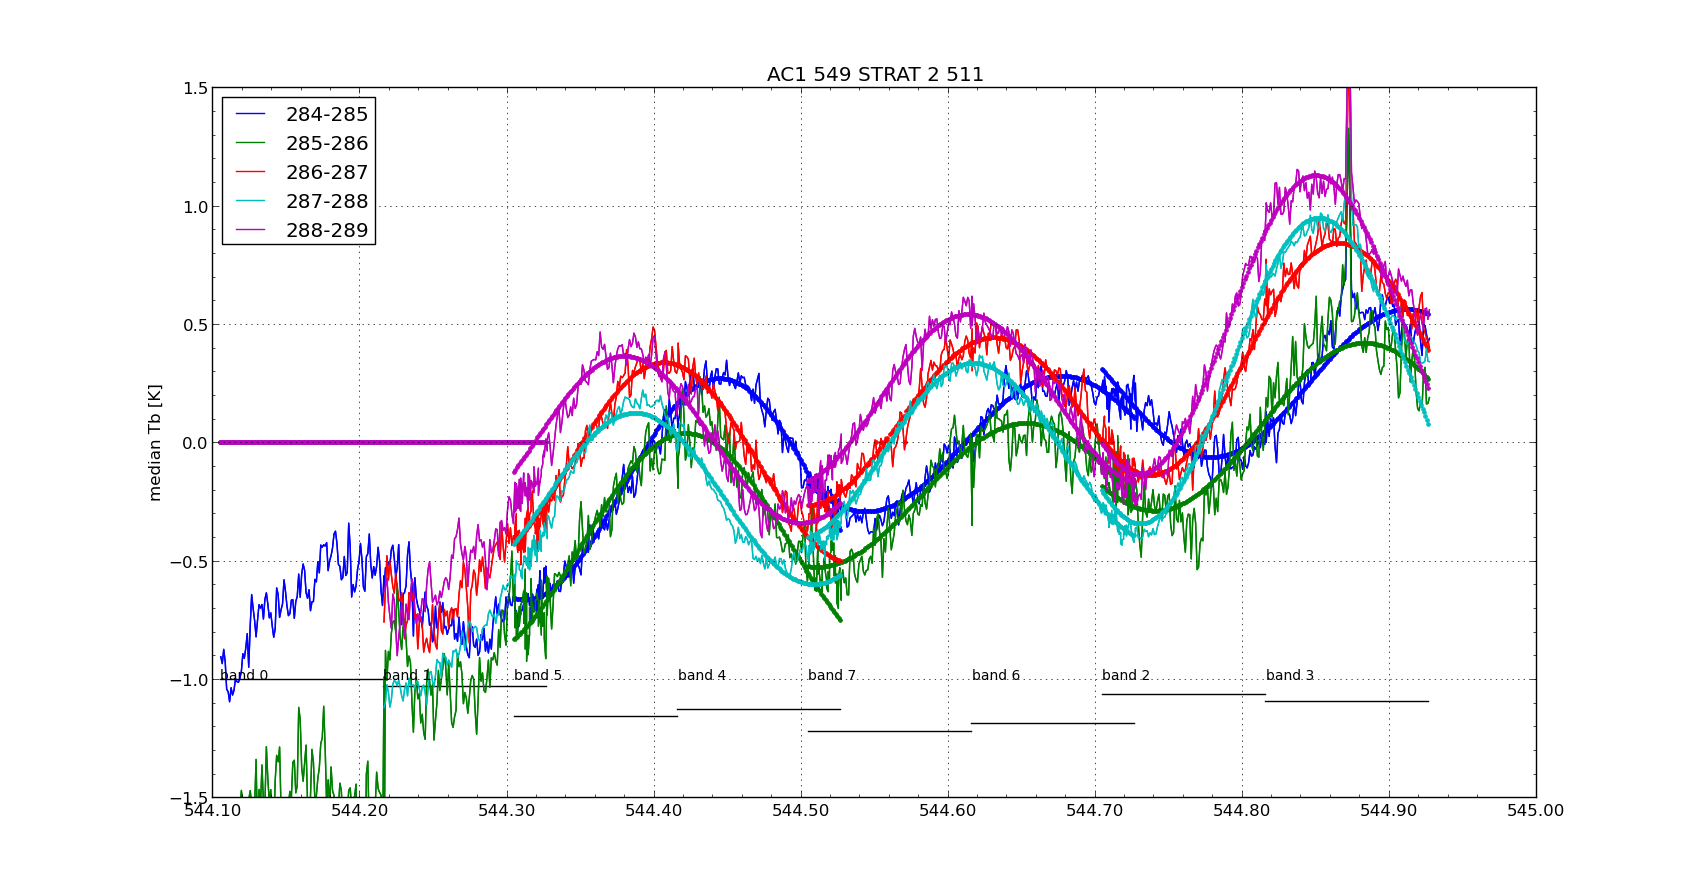
\includegraphics[scale=0.35]{figures/ac1_544_strat2.png}
\caption{Median and fits of calibrated spectra 
(only with calibration Part 1) from 
measurements at high tangent altitudes
 for stratospheric mode 2 of AC1. Data has been grouped into 5 different 
 measurement conditions, where the load
 temperature has been selected to describe the state of the measurements.}
\label{fig:ac1}
\end{figure}


Part 2 of the calibration deals with the removal
of the effects of ripple on the sky signal on calibrated
spectra from part 1, that neglect this effects.
The removal of the artefacts introduced by the sky signal
ripple is a fairly straight forward task, as the artefacts
can be estimated from high tangent point measurements,
where we know that the intensity of a calibrated spectrum should be 0 K.

Ripple on the load signal is more complicated in 
a calibration perspective. The artefacts, in calibrated
atmpospheric spectra, from ripple on the
load signal can be seen as weak signal on top of a strong
atmospheric signal, and thus not easy to detect.
For this reason, we leave this effect unresolved.

Figure~\ref{fig:ac1} shows median spectra of calibrated (Part 1) spectra
from measurements at high tangent altitudes for one of the
observation mode of AC1 (for further discussion on this figure
ignore the most left part of the spectra, which comes from two 
problematic bands of AC1 that should not be used). 
These spectra are expected to be 
centered around 0 K (except for the ozone line between 544.8-544.9 GHz), 
but due to ripple on the sky signal we can see a wave pattern in the spectra.
Figure~\ref{fig:ac1} also indicates that the phase of the wave pattern
depends on the measurement conditions, and the temperature of
the load (ambient temperature) is used in Fig~\ref{fig:ac1}
to describe the measurement condition.


The calibration scheme (Part 2) is as follows:
\begin{itemize}
\item Extract median spectra of calibrated spectra 
(from Part 1:ac\underline{ }level1b table) 
from measurements at tangent altitudes above 80 km for a range of hot load 
temperatures ([277-278 K, 278-279 K, ..., 289-290 K]) 
for each observation mode, and import the spectra
into the ac\underline{ }level1b\underline{ }average table
(Table~\ref{table:ac1c1})
\item Estimate a fit to the median spectrum for each mode, and this is done
by
\begin{enumerate}
\item apply a filter that removes channels, that are contaminated by 
atmospheric information or lines, from the median spectrum 
\item use the target fitting function  
\begin{equation}
y=a+ b\sin(cf+d)
\end{equation}
where \(f\) is the frequency and \(a,b,c,d\) parameters to estimate,
to fit the spectrum for each of the four module of AC1 or AC2.
The fitting is performed in such a way that \(c\) is forced 
to be equal for all of the four module. 
Import the fit into the ac\underline{ }cal\underline{ }level1c
table (Table~\ref{table:ac1b2})
\end{enumerate}
\item Apply the correction.\\
Equation~\ref{correction} is applied to correct a given calibrated 
spectrum (from part 1), where the fit of the median spectrum
with matching hot load temperature range, is used as the \(s_{0}\)
spectrum. 
This is done within the program/functions, described in
Sect.\ref{sec:officialexport}, used to export the official
level1b-product.  
\end{itemize}

      
  



\section{The odincal package}
\subsection{Package details}
A description of the various parts of the package...

\section{Required packages and installation}
This section describes what installation and configuration tasks that have to be completed to install the system from scratch.
\subsection{System preparations}
The installation is done on a Ubuntu 12.04.1 LTS server system. The software suite is designed for python 2.7.

The following packages needs to be installed.
\begin{verbatim}  
  $> sudo apt-get install libpng12-dev python-matplotlib libhdf4-dev
  $> sudo apt-get install python-setuptools python-dev flex bison
  $> sudo apt-get install python-zc.buildout python-numpy libhdf5-serial-dev
  $> sudo apt-get install build-essential postgresql-server-dev-9.1
\end{verbatim}


\subsection{Installation of odincal}

To install the odincal software suite. 

\begin{verbatim}
tar xf odincal-1.0.0.tar.gz
cd odincal-1.0.0
python virtualenv.py .
bin/buildout
\end{verbatim}


\subsection{Postgresql preparation}
Create a database a database called odin owned by your user. (Tip! use your system us
ername for easier access.)
 
\begin{verbatim}  
> sudo -u postgres psql
psql> create user <your_user_name> login;
psql> create database odin owner <your_user_name>;
psql> \q
\end{verbatim}

In a new environment the datamodel must be installed, i.e. create tables and stored functions. To install the datamodel:

\begin{verbatim}  
  $> bin/create_datamodel
\end{verbatim}


\subsection{Automatic downloading from PDC}
Data is downloaded from PDC at KTH to the filesystem locally. This is done with the rsync command using a GSSAPI ticket. A valid kerberos ticket is needed to do this action.

A crontab entry defines the action.
\begin{verbatim}
13 03 * * * rsync -T /tmp -aLKe "ssh -o 'GSSAPIKeyExchange yes'" \
    --log-file=/home/odinop/odincal/rsync.log \
    --exclude-from=/home/odinop/.pdc_excludes \
    donal@pisces.pdc.kth.se:/data/odin/level0/ /misc/pearl/odin/level0/
\end{verbatim}

The --exclude-from refers to a file containing rules for wich directories should be used to syncronisation.

\begin{verbatim}
+ ac1**
+ *.ac1
+ ac2**
+ *.ac2
+ shk**
+ *.shk
+ fba**
+ *.fba
+ att/
+ att/*
+ att_17/
+ att_17/*
+ *.att
- *
\end{verbatim}



\end{document}

